\chapter{Related work\label{related_work}}

\section{Researching type annotations}

One research method to investigate correctness of existing type annotations in Python code is to take a dataset and then run type checking against it \cite{rak-amnouykit_taleoftwo_2020, di_grazia_evolution_2022}. For these type checking runs authors rarely ensure that the type checking tool, type checker version, and the tools settings are a good match to the projects own configuration.

However due to the methodology it is plausible that some of these type errors were false positives. Possible reasons for false positives include: Too strict type checking settings, using different settings from the ones that the project normally uses, and differing type checker version from the ones used.

\comment{TODO: What other type annotation research methodologies were observed in the research material?}


\section{Type annotations}

\section{Usage practices}

Annotations often stay unchanged for a long while after being added \cite{di_grazia_evolution_2022}. Projects can be categorized into three patterns: regular annotation, type sprints, and occasional usage. In a dataset of 9655 Python projects the used pattern correlated with number of contributors, with regular annotation averaging the highest contributor count of 62, type sprints 45, and occasional use projects averaging 25 contributors. A motivation of type annotations helping coordination between higher numbers of active contributors was hypothesized to explain this phenomena. 

\subsection{Popularity}

\begin{figure}
    \centering
    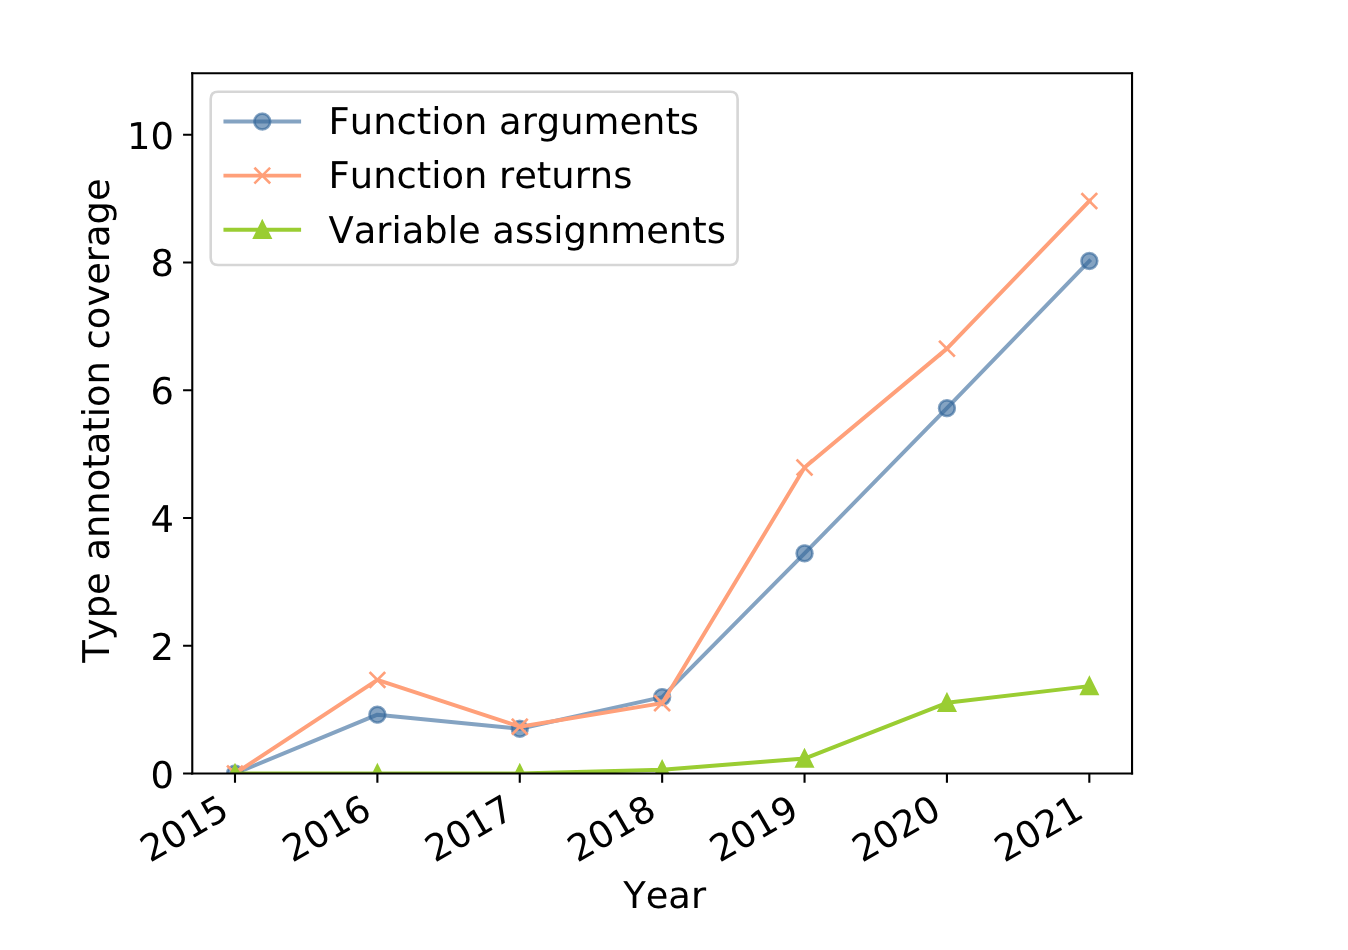
\includegraphics[width=0.5\linewidth]{Screenshot 2024-12-05 at 15.37.59.png}
    \caption{Python Type Annotation evolution from 2015 to 2021 \cite{di_grazia_evolution_2022}}
    \label{fig:annotation-evolution}
\end{figure}
From the introduction of Python type annotations in 2015 they reached around 8\% function argument and return coverage by 2021 in an analysis of 9655 Python projects \cite{di_grazia_evolution_2022}. 

Using a single large Python project picked for representativeness (Tensorflow) \cite{lin_towards_large_scale_2023}, ratio of functions that have type annotations rose from 4.99\% in 2019 to 39.12\% in 2022. This increase seems consistent with the general rate in \ref{fig:annotation-evolution}.

The trend of adoption for type annotations is increasing, but the proportion of typed code was not very high by 2022.

\subsection{Correctness}

A 2020 study of Python type hint usage patterns \cite{rak-amnouykit_taleoftwo_2020} found that even though type hints and checking is more popular, only 15\% of the 2678 codebases analysed successfully type checked with Mypy. They also found out that errors from Mypy and Pytype find both false positives and runtime defect related type errors.

A stduy of 9655 most popular Python projects on Github in 2022 found that 78.3\% of commits that had type annotations contained type errors \cite{di_grazia_evolution_2022}.

\subsection{Empirical benefits}

Making use of types and type checking can allow development time detection of various program defects. In a retroactive analysis it was found that up to 15\% of corrective defects that had to be patched could have been found at development time with types\cite{khan_empirical_2022}. Corrective defects consist of failures in processing, performance and implementation, and thus preventing or fixing them is a necessary part of software maintenance.

Both experienced and inexperienced programmers make significant amounts of type-related mistakes when working with Python \cite{khan_empirical_2022}. These consist of: using variables before initializing them, null safety errors, and re-using variables with values of different types. This implies that both experienced and inexperienced programmers can derive benefits from types, since type checking helps fix these mistakes.


Type annotations can enable improved editor support for the programmer.
\comment{TODO: expand on the editor point, and a citation needed}

\section{Runtime guarantees}

Pydantic is a frequently used data validation library for Python that enables runtime data validation using type annotations\cite{pydanticdev_welcome_nodate}. There is no academic research available on its effectiveness and popularity. Common use cases include web services where incoming data has to be validated anyway, type annotations enabling a simple way to write schemas.

% "observations"
% - Tale of two type systems and TODO reported a high proportion of the used dataset not type checking. (Todo check) They did not report which settings they used when running MyPy and PyType, and it is plausible that they did not configure the type checker version and settings for each source code repository separately. This could cause false false positives, eg errors that do not appear in the repository with correct checker settings. This can also cause errors to appear that are not visible to the project developers, due to being added in a later type checker version than the one they use. 